% !TEX root = saveliev_physics_general_course_2.tex
%!TEX TS-program = pdflatex
%!TEX encoding = UTF-8 Unicode


\chapter[CẢM ỨNG ĐIỆN TỪ]{CẢM ỨNG ĐIỆN TỪ}\label{chap:8}
\chaptermark{CẢM ỨNG ĐIỆN TỪ}

\section{Các hiện tượng cảm ứng điện từ}\label{sec:8_1}

Vào năm 1831, nhà vật lý kiêm hoá học người Anh Michael Faraday (1791-1867) khám phá ra rằng có một dòng điện được sinh ra trong một vòng dây dẫn kín khi từ thông do một nguồn từ trường sinh ra đi qua nó thay đổi. 
Hiện tượng này được gọi là \textbf{cảm ứng điện từ}, và dòng điện sinh ra được gọi là \textbf{dòng điện cảm ứng}.

Hiện tượng cảm ứng điện từ cho biết khi từ thông trong mạch kín biến thiên thì xuất hiện một suất điện động cảm ứng $\ab{\mathcal{E}}{i}$.

Giá trị của $\ab{\mathcal{E}}{i}$ không phụ thuộc vào cách từ thông $\Phi$ thay đổi ra sao mà chỉ được xác định bằng độ biến thiên của $\Phi$ theo thời gian, tức là bằng giá trị của $\diffin{\Phi}{t}$. Sự thay đổi về dấu giá trị của $\diffin{\Phi}{t}$ sẽ quyết định hướng của suất điện động cảm ứng $\ab{\mathcal{E}}{i}$.

Ta xét đến một ví dụ sau đây.
Hình \ref{fig:8_1} là vòng dây dẫn kín $1$ đang có dòng điện $I_1$ có thể điều chỉnh được.
Dòng điện này sẽ tạo ra một từ trường đi qua qua vòng dây kín $2$.
Nếu chúng ta tăng dòng điện $I_1$ thì từ thông $\Phi$ xuyên qua vòng $2$ cũng sẽ tăng lên.
Sự tăng từ thông này sẽ dẫn đến sự xuất hiện trong vòng $2$ một dòng điện cảm ứng $I_2$ được đo bởi điện kế.
Nếu ta giảm dòng điện $I_1$ thì sẽ làm cho từ thông qua vòng $2$ giảm theo.
Điều này sẽ dẫn đến sự xuất hiện trong nó một dòng điện cảm ứng có hướng ngược lại với chiều ban đầu trong trường hợp đầu tiên.
Dòng điện cảm ứng $I_2$ cũng có thể được tạo ra bằng cách đưa vòng $2$ đến gần vòng lặp $1$ hoặc di chuyển nó ra xa.
Trong hai trường hợp này, chiều của dòng điện cảm ứng ngược nhau.
Cuối cùng, cảm ứng điện từ có thể được tạo ra mà không cần chuyển động tịnh tiến của vòng $2$, nhưng bằng cách quay nó để thay đổi góc giữa pháp tuyến của vòng dây và hướng của từ trường.

\begin{figure}[!h]
	\begin{center}
		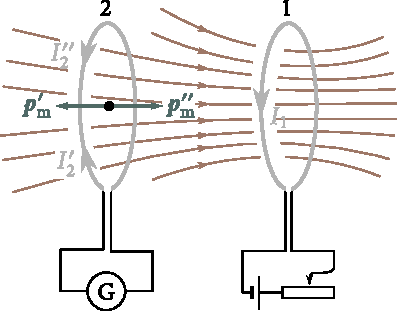
\includegraphics[scale=1]{figures/ch_08/fig_8_1.pdf}
		\caption[]{}
		\label{fig:8_1}
	\end{center}
	\vspace{-0.8cm}
\end{figure}

E. Lenz đã đề ra một quy tắc cho phép chúng ta tìm ra hướng của dòng điện cảm ứng.
\textbf{Quy tắc Lenz} phát biểu rằng một dòng điện cảm ứng luôn có hướng để chống lại nguyên nhân tạo ra nó.
Ví dụ, nếu sự biến thiên $\Phi$ là do chuyển động của vòng $2$, thì một dòng điện cảm ứng được tạo ra theo hướng sao cho lực tương tác từ với vòng $1$ chống lại chuyển động của vòng.
Khi vòng $2$ tiến đến gần vòng $1$ (xem \fig{8_1}), dòng điện $I_2'$ được được tạo ra có mômen từ hướng ngược lại với từ trường do dòng điện $I_1$ sinh ra (góc $\alpha$ giữa các vector $\ab{\vec{p}}{m}'$ và $\vec{B}$ là $\pi$ s).
Do đó, vòng $2$ sẽ chịu một lực đẩy ra xa vòng $1$ [xem \eqn{6_77}].
Khi vòng $2$ di chuyển ra xa khỏi vòng $1$, dòng điện $I_2''$ được sinh ra tạo ra một mômen từ $\ab{\vec{p}}{m}''$ trùng với hướng của từ trường sinh ra bởi dòng điện $I_1$ ($\alpha=0$) do đó lực tác động vào vòng $2$ có hướng hướng về vòng $1$.

Giả sử rằng cả hai vòng đều đứng yên và dòng điện trong vòng $2$ được tạo ra bằng cách thay đổi dòng $I_1$ trong vòng $1$.
Bây giờ dòng điện $I_2$ được tạo ra theo hướng sao cho từ thông mà nó tự tạo ra có xu hướng làm suy yếu sự thay đổi của từ thông bên ngoài dẫn đến thiết lập dòng điện cảm ứng.
Khi $I_1$ tăng lên, tức là, từ thông bên ngoài hướng về bên phải tăng lên, một dòng điện $I_2'$ được tạo ra tạo ra một từ thông hướng sang trái.
Khi $I_1$ giảm đi, dòng điện $I_2''$ được thiết lập mà từ thông nội tại có cùng hướng với từ thông bên ngoài và do đó, có xu hướng giữ cho từ thông bên ngoài không thay đổi.

\section{Suất điện động cảm ứng}\label{sec:8_2}

Chúng ta đã giải thích chung trong phần trước rằng sự thay đổi trong từ thông $\Phi$ qua một vòng kín sẽ thiết lập ra suất điện động cảm ứng $\ab{\mathcal{E}}{i}$ bên trong nó.
Để tìm ra mối liên hệ giữa $\ab{\mathcal{E}}{i}$ và độ biến thiên của $\Phi$, ta xét một ví dụ sau đây.

Ta đặt một thanh thẳng dẫn điện chiều dài $l$ đặt lên một vòng dây sao cho nó có thể chuyển động không ma sát trên vòng dây (\fig{8_2}a).
Ta đặt hệ trong một điện trường đều sao cho vector từ trường vuông góc với mặt phẳng vòng dây.
Tác động vào thanh sao cho nó chuyển động với vận tốc ban đầu $\vec{v}$.
Các hạt tải điện (electron) bên trong thanh sẽ bắt đầu chuyển động tương đối so với từ trường với cùng vận tốc với thanh (kéo theo).
Hệ quả là, mỗi electron sẽ bắt đầu chịu lực từ theo công thức
\begin{equation}\label{eq:8_1}
    \vec{F}_{\parallel} = -e (\vecprod{v}{B}),
\end{equation}

\noindent
có chiều dọc theo thanh [xem \eqn{6_33}; điện tích của electron là $-e$].
Lực này tương đương với một suất điện động tạo ra
\begin{equation*}
    \vec{E} = \vecprod{v}{B}.
\end{equation*}

\noindent
Trường này không có nguồn gốc tĩnh điện. Sự chuyển động thành vòng tuần hoàn của electron sinh ra một suất điện động cảm ứng
\begin{equation}\label{eq:8_2}
    \ab{\mathcal{E}}{i} = \oint \vec{E} \ccdot \derivec{l} = \oint (\vecprod{v}{B}) \ccdot \derivec{l} = \int_1^2 (\vecprod{v}{B}) \ccdot \derivec{l}
\end{equation}

\noindent

Để có thể biết được chiều của suất điện động cảm ứng liên quan đến dấu của $\ab{\mathcal{E}}{i}$, chúng ta sẽ giả sử $\ab{\mathcal{E}}{i}$ có giá trị dương khi chiều của tuân theo quy tắc bàn tay phải.

\begin{figure}[!h]
	\begin{center}
		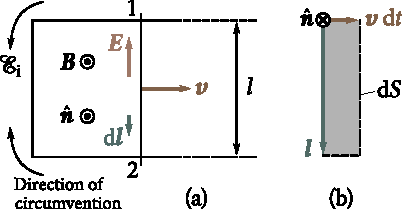
\includegraphics[scale=1]{figures/ch_08/fig_8_2.pdf}
		\caption[]{}
		\label{fig:8_2}
	\end{center}
	\vspace{-0.8cm}
\end{figure}

Chọn chiều pháp tuyến $\hat{\boldsymbol{n}}$ như \fig{8_2}.
Do đó, khi tính toán trên cả vòng kín, chúng ta phải xét vòng theo chiều kim đồng hồ và chọn hướng của vector $\vec{l}$ cho phù hợp.
Nếu chúng ta để vector hằng $\vecprod{v}{B}$ trong \eqn{8_2} ra bên ngoài tích phân, ta sẽ thu được
\begin{equation*}
    \ab{\mathcal{E}}{i} = (\vecprod{v}{B}) \int_1^2 \derivec{l} = (\vecprod{v}{B}) \ccdot \vec{l},
\end{equation*}

\noindent
với $\vec{l}$ là vector được chỉ ra trong \fig{8_2}b.
Sắp xếp lại các nhân tử trong biểu thức thu được, sau đó nhân và chia nó cho $\deriv{t}$:
\begin{equation}\label{eq:8_3}
    \ab{\mathcal{E}}{i} = \vec{B} \ccdot (\vecprod{l}{v}) = \frac{\vec{B} \ccdot (\vec{l} \times \vec{v}\, \deriv{t})}{\deriv{t}}.
\end{equation}

\noindent
Nhìn lướt qua \fig{8_2} b cho thấy 
\begin{equation*}
    \vec{l} \times \vec{v}\, \deriv{t} = - \hatvec{n}\, \deriv{S},
\end{equation*}

\noindent
với $\deriv{S}$ là phần diện tích tăng lên của vòng trong thời gian $\deriv{t}$.
Theo định nghĩa của từ thông,
$\vec{B}\ccdot{\derivec{S}}=\vec{B}\ccdot\hatvec{n}\,\deriv{S}$ là từ thông đi xuyên qua diện tích $\deriv{S}$, tức là, sự tăng lên của từ thông $\deriv{\Phi}$ đi qua vòng dây.
Như vậy,
\begin{equation*}
    \vec{B} \ccdot (\vec{l} \times \vec{v}\, \deriv{t}) = - \vec{B} \ccdot \hatvec{n}\, \deriv{S} = - \deriv{\Phi}.
\end{equation*}

\noindent
Từ biểu thức này, \eqn{8_3} có thể viết dưới dạng
\begin{equation}\label{eq:8_4}
    \ab{\mathcal{E}}{i} = - \diff{\Phi}{t}.
\end{equation}

Ta nhận thấy rằng $\diffin{\Phi}{t}$ và $\ab{\mathcal{E}}{i}$ có dấu giá trị ngược nhau.
Dấu của từ thông và của $\ab{\mathcal{E}}{i}$ liên quan đến việc chọn chiều một pháp tuyến đến mặt phẳng của một vòng dây.
Với việc chọn chiều pháp tuyến như trên (xem \fig{8_2}), dấu của $\diffin{\Phi}{t}$ là dương, và dấu của $\ab{\mathcal{E}}{i}$ là âm.
Nếu chúng ta đã chọn chiều pháp tuyến đi xuyên qua hình vẽ hướng về phía chúng ta, thì dấu của $\diffin{\Phi}{t}$ sẽ là âm và dấu của $\ab{\mathcal{E}}{i}$ sẽ dương.

Đơn vị SI của từ thông cảm ứng là \textbf{weber} (\si{\weber}), định nghĩa là số đường sức từ đi qua \SI{1}{\metre\squared} trong đó các đường sức từ có cảm ứng từ $B = \SI{1}{\tesla}$ trùng với pháp tuyến của mặt diện tích.
Nếu độ biến thiên theo thời gian của từ thông \SI{1}{\weber\per\second}, thì suất điện động cảm ứng \SI{1}{\volt} được sinh ra trong vòng dây.
Trong hệ đơn vị Gauss, \eqn{8_4} có dạng
\begin{equation}\label{eq:8_5}
    \ab{\mathcal{E}}{i} = - \frac{1}{c} \diff{\Phi}{t}.
\end{equation}

\noindent
Đơn vị của $\Phi$ trong hệ này là \textbf{maxwell} (\si{\maxwell}) bằng với từ thông đi qua một diện tích \SI{1}{\centi\metre\squared} với cảm ứng từ $B = \SI{1}{\gauss}$.
Phương trình \eqref{eq:8_5} cho ta $\ab{\mathcal{E}}{i}$
với đơn vị cgse$_U$.
Để đổi sang đơn vị volt, ta nhân kết quả thu được với $300$. vì $300/c = \num{e-8}$, ta có
\begin{equation}\label{eq:8_6}
    \ab{\mathcal{E}}{i}(V) = -\num{e-8}\, \diff{\Phi}{t} \parenthesis{\si{\maxwell\per\second}}.
\end{equation}

Theo lý luận dẫn ta đến \eqn{8_4}, một phần của các ngoại lực duy trì dòng điện trong vòng dây là do sự có mặt của lực từ.
Công của các lực này lên một đơn vị điện tích dương, theo định nghĩa suất điện động, khác 0.
Tình huống này rõ ràng mâu thuẫn với luận điểm được đưa ra trong \sect{6_5} rằng lực từ trường không thể sinh công lên điện tích.
Sự mâu thuẫn này sẽ bị loại bỏ nếu chúng ta tính đến rằng lực \eqref{eq:8_1} không phải là lực từ tổng cộng tác dụng lên một electron, mà chỉ là thành phần của lực này song song với vật dẫn và do vận tốc $\vec{v}$ (xem lực $\vec{F}_{\parallel}$ trong \fig{8_3}).
Thành phần này làm cho êlectron bắt đầu chuyển động dọc theo dây dẫn với vận tốc $\vec{u}$, do đó lực từ vuông góc với dây dẫn và bằng
\begin{equation*}
    \vec{F}_{\parallel} = - e (\vecprod{u}{B})
\end{equation*}

\noindent
(thành phần lực này không đóng góp vào chuyển động thành dòng của electron vì nó vuông góc với $\derivec{l}$).

\begin{figure}[!h]
	\begin{center}
		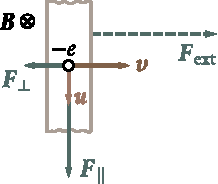
\includegraphics[scale=1]{figures/ch_08/fig_8_3.pdf}
		\caption[]{}
		\label{fig:8_3}
	\end{center}
	\vspace{-0.8cm}
\end{figure}

Lực từ tổng cộng tác dụng lên một electron là
\begin{equation*}
    \vec{F} = \vec{F}_{\parallel} + \vec{F}_{\perp},
\end{equation*}

\noindent
và công của lực này lên một electron trong thời gian $\deriv{t}$ is
\begin{equation*}
    \deriv{A} = \vec{F}_{\parallel} \ccdot \vec{u}\, \deriv{t} + \vec{F}_{\perp} \ccdot \vec{v}\, \deriv{t} = F_{\parallel} u\, \deriv{t} + F_{\perp} v\, \deriv{t}
\end{equation*}

\noindent
(hướng của vector $\vec{F}_{\parallel}$ và $\vec{u}$ là cùng chiều, và của $\vec{F}_{\perp}$ và $\vec{v}$ là ngược chiều; xem \fig{8_3}).
Độ lớn của hai thành phần lực từ là $F_{\parallel}=evB$ và $F_{\perp}=euB$, ta thầy rằng công của cả hai thành phần lực từ bằng không.

Lực $\vec{F}_{\perp}$ có chiều đối ngược so với vận tốc của thanh $\vec{v}$.
Do đó, đối với thanh chuyển động với vận tốc $\vec{v}$, ngoại lực $\ab{\vec{F}}{ext}$ phải đặt vào thanh để cân bằng với tổng lực $\vec{F}_{\perp}$ tác dụng vào toàn bộ electron tự do có trong thanh.
Chính xác là do tác dụng của lực này mà năng lượng được giải phóng trong vòng dây bởi dòng điện cảm ứng sẽ được tạo ra.

Giải thích về sự xuất hiện của suất điện động cảm ứng liên quan đến trường hợp khi từ trường không đổi, trong khi hình dạng của vòng thay đổi.
Tuy nhiên, từ thông qua vòng lặp cũng có thể được thay đổi bằng cách thay đổi $\vec{B}$. Trong trường hợp này, lời giải thích về sự xuất hiện của suất điện động cảm ứng sẽ khác nhau về nguyên tắc.
Từ trường thay đổi theo thời gian sẽ tạo ra một điện trường xoáy $\vec{E}$ (điều này được giải thích chi tiết trong \sect{9_1}).
Tác động của điện trường $\vec{E}$ làm cho các hạt tải điện trong một vật dẫn bắt đầu chuyển động --- một dòng điện cảm ứng được tạo ra.
Mối quan hệ giữa suất điện động cảm ứng và sự biến thiên từ thông trong trường hợp này cũng được mô tả bởi \eqn{8_4}.

Giả sử vòng dây có suất điện động cảm ứng bao gồm $N$ vòng thay vì chỉ một vòng, tức là, nó là một solenoid.
Bởi vì các vòng dây được nối tiếp với nhau, $\ab{\mathcal{E}}{i}$ sẽ bằng với tổng của suất điện động cảm ứng được tạo ra bởi mỗi vòng dây:
\begin{equation*}
    \ab{\mathcal{E}}{i} = - \sum \diff{\Phi}{t} = - \diff{}{t}\parenthesis{\sum \Phi}.
\end{equation*}

Đại lượng
\begin{equation}\label{eq:8_7}
    \Psi = \sum \Phi,
\end{equation}

\noindent
được gọi là \textbf{từ thông liên kết} hay \textbf{từ thông tổng cộng}. Đơn vị cúa nó giống với đơn vị của $\Phi$.
Nếu từ thông đi qua các vòng dây là như nhau, thì
\begin{equation}\label{eq:8_8}
    \Psi = N \Phi.
\end{equation}

\noindent
Suất điện động cảm ứng sinh ra trong solenoid đó được xác định bởi
\begin{equation}\label{eq:8_9}
    \ab{\mathcal{E}}{i} = - \diff{\Psi}{t}.
\end{equation}

\section{Phương pháp đo cảm ứng từ}\label{sec:8_3}

Giả sử rằng tổng từ thông của một vòng dây thay đổi từ $\Psi_1$ thành $\Psi_2$.
Hãy tìm điện tích $q$ chạy qua mỗi phần của vòng dây.
Giá trị tức thời của cường độ dòng điện trong mạch vòng là
\begin{equation*}
	I = \frac{\mathcal{E}}{R} = - \frac{1}{R} \diff{\Psi}{t}.
\end{equation*}

\noindent
Từ đó,
\begin{equation*}
	\deriv{q} = I\, \deriv{t} = - \frac{1}{R} \diff{\Psi}{t}\, \deriv{t} = - \frac{1}{R}\, \deriv{\Psi}.
\end{equation*}

\noindent
Tích phân biểu thức này tạo ra tổng điện tích:
\begin{equation}\label{eq:8_10}
	q = \int \deriv{q} = - \frac{1}{R} \int_1^2 \deriv{\Psi} = \frac{1}{R} (\Psi_1 - \Psi_2).
\end{equation}

Phương trình \eqref{eq:8_10} làm cơ sở cho phương pháp đo cảm ứng từ được phát triển bởi A. Stoletov.
Nó bao gồm những điều sau đây.
Một cuộn dây nhỏ có $N$ vòng được đặt trong một từ trường đang xét.
Cuộn dây được bố trí sao cho vector $\vec{B}$ vuông góc với mặt phẳng của các vòng dây (\fig{8_4} a).
Do đó, tổng từ thông đi qua cuộn dây sẽ là
\begin{equation*}
	\Psi_1 = NBS,
\end{equation*}

\noindent
trong đó $S$ là diện tích của một vòng, phải nhỏ đến mức 
từ trường đi quá có thể giới hạn coi là đồng nhất đều.

\begin{figure}[!h]
	\begin{center}
		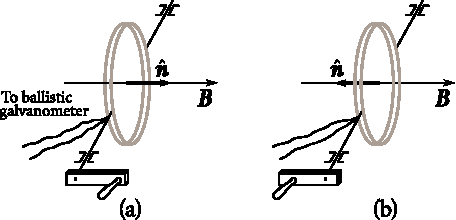
\includegraphics[scale=1]{figures/ch_08/fig_8_4.pdf}
		\caption[]{}
		\label{fig:8_4}
	\end{center}
	\vspace{-0.8cm}
\end{figure}

Khi quay cuộn dây $180$ độ (\fig{8_4}b), từ thông qua cuộn dây bằng $\Psi_2=-NBS$ ($\hatvec{n}$ và $\vec{B}$ là ngược chiều nhau).
Do đó, sự thay đổi từ thông tổng cộng qua cuộn dây sau khi quay là $\Psi_1 - \Psi_2 = 2NBS$. Nếu cuộn dây quay đủ nhanh, một xung điện tích được tạo ra trong vòng dây với độ lớn
\begin{equation}\label{eq:8_11}
	q = \frac{1}{R} 2NBS
\end{equation}

\noindent
chạy qua [xem \eqn{8_10}].

Điện tích chạy trong mạch có thể được đo bởi một máy đo gọi là \textbf{điện kế xung kích}.
Sau đó là một điện kế có chu kỳ dao động riêng rất lớn.
Sau khi đo được $q$ và biết được giá trị của $R$, $N$, và $S$, chúng ra sẽ tìm được $B$ theo \eqn{8_11}.
Ở đây, $R$ là điện trở của toàn bộ mạch bao gồm cuộn dây, các dây nối và điện kế.

Thay vì quay cuộn dây, chúng ta có thể bật (hoặc tắt) từ trường đang được nghiên cứu, hoặc đảo ngược hướng của nó.

Để đo $B$, trường hợp cũng được sử dụng là điện trở của bismuth tăng lên rất nhiều dưới tác dụng của từ trường --- khoảng năm phần trăm của một phần mười tesla (mỗi \SI{1000}{\gauss}).
Do đó, chúng ta có thể xác định cảm ứng từ của từ trường bằng cách đặt một cuộn dây bismuth được chia độ (\fig{8_5}) vào trong từ trường và đo sự thay đổi tương đối trong điện trở của nó.

Chúng ta phải lưu ý rằng điện trở của các kim loại khác cũng tăng lên khi trong từ trường, nhưng ở một mức độ nhỏ hơn nhiều.
Ví dụ, đối với đồng, mức tăng điện trở bằng khoảng một phần mười nghìn so với bismuth.

\section{Dòng điện Eddy}\label{sec:8_4}

Dòng điện cảm ứng cũng có thể được tạo ra trong các vật dẫn rắn có khối lượng lớn.
Trong trường hợp này chúng được gọi là \textbf{dòng điện Eddy}.
Điện trở của một vật dẫn lớn nhỏ, do đó, dòng điện Eddy có thể đạt giá trị rất cao.

\begin{figure}[!h]
	\begin{minipage}[t]{0.48\linewidth}
		\begin{center}
			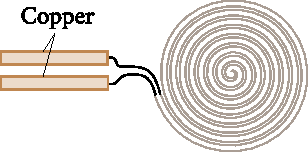
\includegraphics[scale=1]{figures/ch_08/fig_8_5.pdf}
			\caption[]{}
			\label{fig:8_5}
		\end{center}
	\end{minipage}
	\hfill{ }%space{-0.05cm}
	\begin{minipage}[t]{0.48\linewidth}
		\begin{center}
			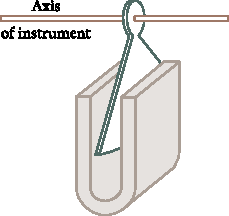
\includegraphics[scale=1]{figures/ch_08/fig_8_6.pdf}
			\caption[]{}
			\label{fig:8_6}
		\end{center}
	\end{minipage}
\vspace{-0.4cm}
\end{figure}

Theo quy tắc Lenz, dòng điện Eddy chọn các đường đi và hướng trong một vật dẫn sao cho nó có xu hướng chống lại nguyên nhân sinh ra nó càng nhiều càng tốt.
Đây là lý do tại sao các vật dẫn chuyển động trong một từ trường mạnh bị chậm lại do sự tương tác của dòng điện xoáy với từ trường.
Nguyên lý này được áp dụng để giảm chấn các bộ phận chuyển động của điện kế, máy đo địa chấn, và phổ biến nhất là phanh từ trong các loại phương tiện, thay thế cho các phanh ma sát.
Một tấm dẫn phẳn (ví dụ, nhôm, đồng) được gắn chặt vào bộ phận có thể chuyển động của một dụng cụ (\fig{8_6}) và được đưa vào khe giữa các cực của một nam châm vĩnh cửu mạnh hình chữ U.
Chuyển động của tấm làm cho dòng điện Eddy được tạo ra trong nó, và tác dụng với từ trường của nam châm và hãm chuyển động của hệ thống.
Ưu điểm của một thiết bị như vậy là tác động phanh chỉ xuất hiện khi đĩa chuyển động và biến mất khi đĩa đứng yên.
Do đó, phanh từ hoàn toàn không cản trở thiết bị đến vị trí cân bằng của nó một cách chính xác.

Tác dụng nhiệt của dòng điện Eddy còn được dùng trong công nghiệp luyện kim, cụ thể là lò nung từ.
 Một lò nung từ bao gồm một cuộn dây được cấp một dòng điện tần số cao có giá trị lớn.
Nếu chúng ta đặt một vât dẫn điện bên trong cuộn dây, dòng điện Eddy mạnh sẽ được tạo ra bên trong vật dẫn và
có thể làm nóng nó đến nhiệt độ nóng chảy.
Phương pháp này dùng để nấu chảy kim loại trong chân không.
Các vật liệu sau nóng chảy có độ tinh khiết cực cao.

Dòng điện xoáy cũng được sử dụng để làm nóng các thành phần kim loại bên trong của hệ thống chân không để tẩy dầu mỡ cho chúng.

Dòng điện Eddy thường không mong muốn và phải thực hiện các biện pháp đặc biệt để loại bỏ chúng.
Ví dụ, để tránh thất thoát năng lượng cho việc làm nóng lõi máy biến áp bởi dòng điện Eddy, các lõi được ghép bằng các tấm cách điện mỏng. Lõi biến áp thường được sản xuất bằng ferrrite (vật liệu từ tính bán dẫn có điện trở cao) để giảm thiểu tối đa hiệu ứng dòng Eddy.

Dòng điện Eddy được thiết lập trong vật dẫn mang dòng điện xoay chiều được định hướng để làm suy yếu dòng điện bên trong vật dẫn và phân bố dòng điện lên gần bề mặt.
Kết quả là, dòng điện thay đổi nhanh chóng được phân bố
không đều trên tiết diện của dây dẫn --- nó bị ép ra bề mặt của dây dẫn.
Hiện tượng này được gọi là \textbf{hiệu ứng bề mặt} (\textit{skin effect}).
Do hiệu ứng này xảy ra, phần bên trong của dây dẫn trong mạch tần số cao bị triệt tiêu. Đây là lý do tại sao các dây dẫn được sử dụng cho các mạch như vậy có dạng ống rỗng, để tiết kiệm chi phí nguyên liệu và giảm khối lượng chế tạo dây điện.

\section{Hiện tượng tự cảm}\label{sec:8_5}

Một dòng điện $I$ chạy trong một vòng dây dẫn kín sẽ tạo ra một từ trường, và chính từ trường này đi xuyên qua vòng dây tạo ra một từ thông $\Psi$.
Khi $I$ thay đổi, $\Psi$ cũng thay đổi, và kết quả là một suất điện động cảm ứng được sinh ra trong vòng dây.
Hiện tượng này được gọi là \textbf{tự cảm}.
Theo định luật Biot-Savart, cảm ứng từ $B$ tỉ lệ với cường độ dòng điện thiết lập từ trường.
Do đó, dòng điện $I$ trong vòng dây và từ thông $\Psi$ qua vòng dây mà nó tạo ra tỷ lệ thuận với nhau:
\begin{equation}\label{eq:8_12}
	\Psi = L I.
\end{equation}

\noindent
Hệ số tỉ lệ $L$ giữa cường độ dòng điện và từ thông được gọi là \textbf{độ tự cảm} của một vòng dây.

Ta chỉ quan sát thấy sự phụ thuộc tuyến tính của $\Psi$ vào $I$ nếu độ từ thẩm $\mu$ của môi trường xung quanh vòng dây không phụ thuộc vào cường độ từ trường $H$, tức là không có sự xuất hiện của sắt từ
Nếu không, $\mu$ sẽ là một hàm phụ thuộc vào $I$ (theo $H$, xem \fig{7_19}b), và, vì $B=\mu_0\mu H$, sự phụ thuộc của $\Psi$ vào $I$ cũng sẽ khá phức tạp.
Phương trình \eqref{eq:8_12}, tuy nhiên, cũng được mở rộng cho trường hợp này, và độ tự cảm $L$ được coi là một hàm của $I$.
Đối với đòng điện không đổi $I$, từ thông tổng cộng $\Psi$ có thể thay đổi do sự thay đổi hình dạng của vòng dây.

Từ trên có thể thấy rằng độ tự cảm $L$ phụ thuộc vào dạng hình học của một vòng dây (tức là, về hình dạng và kích thước của nó), và cả về tính chất từ tính ($\mu$) của môi trường xung quanh vòng dây.
Nếu vòng dây là cứng và không có chất sắt từ gần nó thì độ tự cảm $L$ là một đại lượng không đổi.
Đơn vị SI của độ tự cảm là độ tự cảm của một vật dẫn trong đó tổng từ thông $\Psi$ là \SI{1}{\weber} tạo ra bởi dòng điện $I$ có giá trị \SI{1}{\ampere} bên trong dây dẫn. Đơn vị này được gọi là \textbf{henry} (\si{\henry}).

Trong hệ đơn vị Gauss, độ tự cảm có thứ nguyên là độ dài.
Theo đó, đơn vị của độ tự cảm trong hệ này là
được gọi là \textbf{centimetre}.
Một vòng dây có từ thông \SI{1}{\maxwell} (\SI{e-8
}{\weber}) tạo ra bởi dòng điện \SI{1}{\cgs{m}{I}} (\ie, \SI{10}{\ampere}) có độ tự cảm \SI{1}{\centi\metre}.

Bây giờ ta sẽ tính độ tự cảm của một cuộn dây solenoid.
Chúng ta sẽ sử dụng một solenoid dài đến mức có thể coi là vô hạn
Khi dòng điện $I$ chạy bên trong solenoid, một từ trường gần như là đều được tạo ra bên trong ống solenoid với cảm ứng từ $B=\mu_0\mu nI$ [xem \eqns{6_108}{7_26}].
Từ thông đi qua mỗi vòng dây là $\Phi=BS$, và từ thông tổng cộng đi qua solenoid là
\begin{equation}\label{eq:8_13}
	\Psi = N\Phi = nlBS = \mu_0 \mu n^2 l S I,
\end{equation}

\noindent
với $l$ là độ dài của solenoid (được coi là rất lớn), $S$ là tiết diện, và $n$ số vòng dây trên một đơn vị chiều dài (tích $nl$ sẽ cho ta tổng số vòng dây $N$).

Từ hai phương trình \eqn{8_12} và \eqn{8_13} cho ta biểu thức của độ tự cảm của solenoid dài
\begin{equation}\label{eq:8_14}
	L = \mu_0 \mu n^2 l S = \mu_0 \mu n^2 V,
\end{equation}

\noindent
với $V = lS$ là thể tích của ống solenoid.

Từ phương trình \eqn{8_14} thứ nguyên của $\mu_0$ là thứ nguyên của độ tự cảm chia cho thứ nguyên độ dài.
Do đó, $\mu_0$ được có đơn vị là H/m [xem \eqn{6_3}].

Khi dòng điện trong vòng dây thay đổi, một suất điện động tự cảm $\ab{\mathcal{E}}{s}$ được tạo ra
\begin{equation}\label{eq:8_15}
	\ab{\mathcal{E}}{s} = - \diff{\Psi}{t} = - \diff{(LI)}{t} = - \parenthesis{L\, \diff{I}{t} + I\, \diff{L}{t}}.
\end{equation}

\noindent
Nếu độ tự cảm không đổi khi dòng điện thay đổi (điều này chỉ có thể xảy ra khi không có chất sắt từ), biểu thức cho suất điện động tự cảm trở thành
\begin{equation}\label{eq:8_16}
	\ab{\mathcal{E}}{s} = - L\, \diff{I}{t}.
\end{equation}

\noindent
Dấu trừ trong \eqn{8_16} là do quy tắc Lenz, theo đó dòng điện cảm ứng có hướng để chống lại nguyên nhân tạo ra nó.
Đối với trường hợp đang xét, nguyên nhân tạo ra $\ab{\mathcal{E}}{s}$ là sự thay đổi $I$ trong vòng dây.
Chúng ta hãy giả sử quy ước chiều kim đồng hồ là chiều dương.
Trong những điều kiện này, dòng điện sẽ lớn hơn 0 nếu nó chạy theo chiều kim đồng hồ trong mạch và nhỏ hơn 0 nếu nó chạy ngược chiều kim đồng hồ.
Tương tự, $\ab{\mathcal{E}}{s}$ sẽ lớn hơn
0 nếu nó được tác động theo chiều kim đồng hồ và nhỏ hơn 0 nếu nó được tác động theo chiều ngược kim đồng hồ.

Giá trị của $\diffin{I}{t}$ sẽ dương trong hai trường hợp---hoặc khi dòng điện dương tăng lên hoặc khi giảm giá trị tuyệt đối của dòng điện âm.
Việc kiểm tra \eqn {8_16} cho thấy rằng trong những trường hợp này $\ab{\mathcal{E}}{s}<0$.
Điều này cho thấy rằng suất điện động tự cảm hướng ngược chiều kim đồng hồ và do đó ngược với sự biến thiên dòng điện ở trên.

Giá trị của $\diffin{I}{t}$ sẽ âm trong hai trường hợp---hoặc khi cường độ dòng điện dương giảm đi hoặc khi cường độ dòng điện âm tăng lên. Trong hai trường hợp, $\ab{\mathcal{E}}{s}>0$ và do đó, ngược lại với chiều biến thiên dòng điện.

Phương trình \eqref{eq:8_16} tạo sự khả thi để có thể xác định độ tự cảm là một hằng số tỷ lệ giữa tốc độ thay đổi của dòng điện trong một vòng dây và suất điện động tự cảm.
Quy ước như vậy là đúng, tuy nhiên chỉ khi $L=\text{constant}$.
Nếu có sự xuất hiện của sắt từ, $L$ sẽ là một hàm phụ thuộc vào $I$ (qua $H$).
Do đó, $\diffin{L}{t}$ có thể được viết thành $(\diffin{L}{I})(\diffin{I}{t})$.
Thay vào phương trình \eqn{8_15}, ta thu được
\begin{equation}\label{eq:8_17}
	\ab{\mathcal{E}}{s} = - \parenthesis{L + I\, \diff{L}{I}}\, \diff{I}{t}.
\end{equation}

\noindent
Dễ thấy rằng nếu có sự xuất hiện của sắt từ thì hằng số tỉ lệ giữa $\diffin{I}{t}$ và $\ab{\mathcal{E}}{s}$ không bằng $L$.

\section{Dòng điện khi mạch đóng và mở}\label{sec:8_6}

Theo quy tắc Lenz, các dòng điện bổ sung được thiết lập do hiện tượng tự cảm ứng luôn có hướng để ngăn chặn bất kỳ sự thay đổi nào của dòng điện trong mạch.
Kết quả là dòng điện tăng đến giá trị ổn định khi đóng mạch hoặc giảm xuống 0 khi mở mạch không phải ngay lập tức mà là thay đổi từ từ.

Chúng ta sẽ đầu tiên nghiên cứu xem dòng điện trong một đoạn mạch thay đổi như thế nào khi công tắc mở.
Lắp một mạch điện như (\fig{8_7}).
Dòng điện khi ổn định chạy trong mạch có giá trị
\begin{equation}\label{eq:8_18}
	I_0 = \frac{\mathcal{E}}{R}
\end{equation}

\noindent
(ta có thể bỏ qua điện trở trong của nguồn điện).

\begin{figure}[!h]
	\begin{center}
		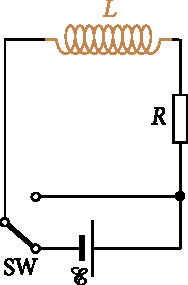
\includegraphics[scale=1]{figures/ch_08/fig_8_7.pdf}
		\caption[]{}
		\label{fig:8_7}
	\end{center}
	\vspace{-0.8cm}
\end{figure}

Tại thời điểm $t=0$, ta ngắt nguồn điện và nối ngắn mạch.
Ngay khi dòng điện bắt đầu giảm, một suất điện động tử cảm xuất hiện ngăn chặn sự giảm dòng điện trong mạch.
Dòng điện trong mạch sẽ tuân theo phương trình
\begin{equation*}
	IR = \ab{\mathcal{E}}{s} = - L \diff{I}{t},
\end{equation*}

\noindent
hay
\begin{equation}\label{eq:8_19}
	\diff{I}{t} + \frac{R}{L} I = 0.
\end{equation}

\noindent
Phương trình \eqref{eq:8_19} là một phương trình vi phân tuyến tính thuần nhất cấp một.
Phân ly biến số, ta có
\begin{equation*}
	\frac{\deriv{I}}{I} = - \frac{R}{L}\, \deriv{t},
\end{equation*}

\noindent
nguyên hàm lên ta được
\begin{equation*}
	\ln{I} = - \frac{R}{L} t + \ln(\text{constant})
\end{equation*}

\noindent
Biến đổi tiếp ta thu được hàm của $I$ theo $t$
\begin{equation}\label{eq:8_20}
	I = \text{constant} \times \exp\parenthesis{- \frac{R}{L} t}.
\end{equation}

\noindent
Phương trình \eqref{eq:8_20} là một nghiệm tổng quát của phương trình \eqn{8_19}.
Hằng số được xác định bởi các điều kiện ban đầu
Tại thời điểm $t=0$, giá trị của cường độ dòng điện là \eqn{8_18}.
Do đó, $\text{constant}=I_0$.
Lắp vào \eqn{8_20}, cuối cùng ta thu được
\begin{equation}\label{eq:8_21}
	I = I_0\, \exp\parenthesis{- \frac{R}{L} t}.
\end{equation}

Như vậy, sau khi nguồn điện bị ngắt, dòng điện trong mạch không biến mất ngay lập tức mà giảm dần theo hàm mũ theo phương trình \eqref{eq:8_21}.
Đồ thị hàm $I$ theo thời gian được mô tả ở \fig{8_8} (đường cong $1$).
Độ giảm dòng điện được xác định bởi
\begin{equation}\label{eq:8_22}
	\tau = \frac{L}{R},
\end{equation}

\noindent
có thứ nguyên thời gian và được gọi là \textbf{thời gian riêng} của mạch điện.
Thay $1/\tau$ vào $R/L$ trong \eqn{8_21}, ta được
\begin{equation}\label{eq:8_23}
	I = I_0\, \exp\parenthesis{- \frac{t}{\tau}}.
\end{equation}

\begin{figure}[!h]
	\begin{center}
		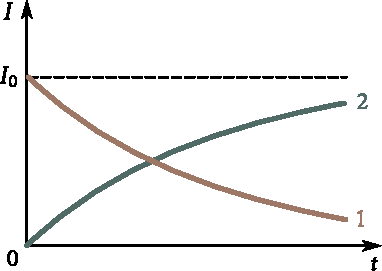
\includegraphics[scale=1]{figures/ch_08/fig_8_8.pdf}
		\caption[]{}
		\label{fig:8_8}
	\end{center}
	\vspace{-0.8cm}
\end{figure}

\noindent
Theo như phương trình trên, $\tau$ là thời gian dòng điện trong mạch giảm $1/e$-th lần so với giá trị ban đầu.
Nhìn lướt qua \eqn{8_22} ta thấy thời gian riêng $\tau$ tăng và dòng điện trong mạch giảm chậm khi độ tự cảm $L$ tăng hoặc điện trở $R$ giảm.

Để đơn giản hóa tính toán , ta coi rằng mạch bị ngắn mạch khi nguồn bị ngắt.
Nếu chúng ta chỉ đơn giản là ngắt mạch điện bằng một cuộn cảm có độ tự cảm cao, thì điện áp cảm ứng cao được thiết lập sẽ tạo ra tia lửa điện hoặc hồ quang tại nơi cắt mạch điện.

Bây giờ ta sẽ xét khi mạch đóng.
Sau khi nguồn điện được bật lên, một suất điện động tự cảm sẽ xuất hiện ngược chiều và cản trở sự tăng dòng điện trong mạch và dòng sẽ tăng từ từ đến giá trị \eqn{8_18}.
Theo định luật Ohm
\begin{equation*}
	IR = \mathcal{E} + \ab{\mathcal{E}}{s} + \mathcal{E} - L\, \diff{I}{t},
\end{equation*}

\noindent
hay
\begin{equation}\label{eq:8_24}
	\diff{I}{t} + \frac{R}{L} I = \frac{\mathcal{E}}{L}.
\end{equation}

Chúng ta đã đi đến một phương trình vi phân tuyến tính không thuần nhất chỉ khác với \eqn{8_19} ở chỗ bên phải chứa đại lượng không đổi $\mathcal{E}/L$ thay vì 0.
Theo lý thuyết về phương trình vi phân, nghiệm tổng quát của một phương trình không thuần nhất tuyến tính có thể nhận được bằng cách thêm bất kỳ nghiệm riêng nào của nó vào nghiệm tổng quát của phương trình thuần nhất tương ứng (xem Phần 7.4 của Tập I).
Nghiệm tổng quá của phương trình vi phân tuyến tính thuần nhất được đưa ra ở \eqn{8_20}.
Dễ thấy rằng $I=\mathcal{E}/R=I_0$ là một nghiệm riêng của \eqn{8_24}.
Do đó, hàm
\begin{equation*}
	I = I_0 + \text{constant} \times \exp\parenthesis{- \frac{R}{L} t},
\end{equation*}

\noindent
là nghiệm tổng quát của \eqn{8_24}.
Tại thời điểm ban đầu, dòng điện trong mạch là không
Do đó, $\text{constant}=-I_0$, và
\begin{equation}\label{eq:8_25}
	I = I_0 \bracket{1 - \exp\parenthesis{ -\frac{R}{L} t}}.
\end{equation}

\noindent
Hàm này mô tả sự tăng lên từ từ của dòng điện trong mạch sau khi nguồn điện đóng. 
Hàm \eqref{eq:8_25} được mô tả ở đồ thị trên \fig{8_8} (đường cong $2$).

\section{Hiện tượng hỗ cảm}\label{sec:8_7}

Ta đặt vòng dây $1$ và $2$ sát lại gần nhau (\fig{8_9}).
Nếu có dòng điện $I_1$ chạy trong vòng $1$, nó sẽ tạo ra một từ thông đi qua vòng $2$ tỉ lệ thuận với $I_1$, \ie,
\begin{equation}\label{eq:8_26}
	\Psi_2 = L_{21} I_1
\end{equation}

\noindent
(trường tạo ra thông lượng này được mô tả trong hình bằng các đường liền nét).
Khi dòng $I_1$ biến thiên, một suất điện động cảm ứng.
\begin{equation}\label{eq:8_27}
	\ab{\mathcal{E}}{i,$2$} = - L_{21}\, \diff{I_1}{t},
\end{equation}

\noindent
được tạo ra trong vòng $2$ (giả sử rằng không có sắt từ gần các vòng).

\begin{figure}[!h]
	\begin{center}
		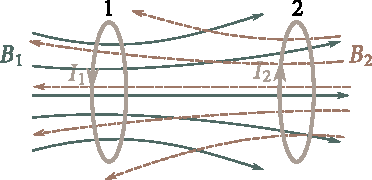
\includegraphics[scale=1]{figures/ch_08/fig_8_9.pdf}
		\caption[]{}
		\label{fig:8_9}
	\end{center}
	\vspace{-0.8cm}
\end{figure}

Tương tự, khi có dòng điện $I_2$ chạy trong vòng $2$ thì sẽ có từ thông đi qua vòng $1$:
\begin{equation}\label{eq:8_28}
	\Psi_1 = L_{12} I_2
\end{equation}

\noindent
(trường tạo ra thông lượng này được mô tả trong hình bằng các đường nét đứt).
Khi dòng $I_2$ biến thiên, một suất điện động cảm ứng
\begin{equation}\label{eq:8_29}
	\ab{\mathcal{E}}{i,$1$} = - L_{12}\, \diff{I_2}{t},
\end{equation}

\noindent
được tạo ra trong vòng $1$.

Vòng $1$ và $2$ are được gọi là \textbf{cặp xung đối}, trong khi hiện tượng thiết lập suất điện động cảm ứng trong một trong các vòng khi những biến thiên về dòng điện trong vòng khác được gọi là \textbf{hỗ cảm}.

Các hệ số tỉ lệ $L_{12}$ và $L_{21}$ được gọi là \textbf{độ hỗ cảm} của các vòng dây.
Các tính toán liên quan cho thấy rằng trong trường hợp không có sắt từ, các hệ số này luôn bằng nhau:
\begin{equation}\label{eq:8_30}
	L_{12} = L_{21}.
\end{equation}

\noindent
Độ lớn của chúng phụ thuộc vào hình dạng, kích thước,
và sự sắp xếp lẫn nhau của các vòng, và cả về tính từ thấm của môi trường xung quanh các vòng.
Đại lượng $L_{12}$ có thứ nguyên trùng với độ tự cảm $L$.

Ta sẽ đi tìm độ hỗ cảm của hai cuộn dây quấn vào chung một lõi sắt hình xuyến (\fig{8_10}).
Các đường cảm ứng từ phân bố chủ yếu bên trong lõi [đọc đoạn văn liên quan đến \eqn{7_31}].
Do đó, chúng ta có thể coi rằng từ trường được thiết lập bởi bất kỳ cuộn dây nào sẽ có cùng cường độ trong suốt lõi.
Nếu cuộn dây thứ nhất có $N_1$ vòng và mang dòng điện $I_1$ chạy trong nó, theo định lý Ampere [xem \eqn{7_11}], ta có
\begin{equation}\label{eq:8_31}
	Hl = N_1 I_1
\end{equation}

\noindent
(ở đây, $l$ là độ dài của cuộn dây).

\begin{figure}[!h]
	\begin{center}
		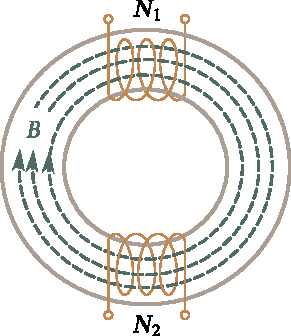
\includegraphics[scale=1]{figures/ch_08/fig_8_10.pdf}
		\caption[]{}
		\label{fig:8_10}
	\end{center}
	\vspace{-0.8cm}
\end{figure}

Từ thông đi qua tiết diện của lõi là $\Phi=BS=\mu_0\mu HS$, với $S$ là tiết diện của lõi.
 Từ \eqn{8_31} và nhân với $N_2$, ta thu được tổng từ thông đi qua cuộn dây thứ hai:
\begin{equation*}
	\Psi_2 = \frac{S}{l} \mu_0 \mu N_1 N_2 I_1.
\end{equation*}

\noindent
So sánh phương trình trên với \eqn{8_26} ta thấy
\begin{equation}\label{eq:8_32}
	L_{21} = \frac{S}{l} \mu_0 \mu N_1 N_2.
\end{equation}

Tương tự ta sẽ có
\begin{equation}\label{eq:8_33}
	L_{12} = \frac{S}{l} \mu_0 \mu N_1 N_2,
\end{equation}

\noindent
ta thấy $L_{21} = L_{12}$.
Trong một vài trường hợp đặc biệt, ta không thể khẳng định rằng $L_{12}=L_{21}$. Nhân tử $\mu$ trong biểu thức phụ thuộc vào cường độ từ trường $H$ bên trong lõi.
Nếu $N_1\neq N_2$, thì cùng một dòng điện đi qua một lần qua cuộn thứ nhất và một lần khác qua cuộn thứ hai sẽ thiết lập một trường có cường độ $H$ khác nhau trong lõi.
Theo đó, các giá trị của $\mu$ trong cả hai trường hợp sẽ khác nhau khi $I_1=I_2$ thì giá trị số của $L_{12}$ và $L_{21}$ sẽ không trùng nhau.

\section{Năng lượng từ trường}\label{sec:8_8}

Xét mạch như \fig{8_11}.
Khi khoá đóng, dòng $I$ sẽ đươc tạo ra bên trong ống solenoid.
Nó sẽ tạo ra một từ trường gần đề bên trong lòng ống.
Nếu khoá mở, một dòng điện giảm dần đều sẽ chạy qua điện trở $R$.
Dòng này được duy trì bởi suất điện động tự cảm bên trong cuộn dây solenoid.
Công của dòng điện trong thời gian $\deriv{t}$ là
\begin{equation}\label{eq:8_34}
	\deriv{A} = \ab{\mathcal{E}}{s} I\, \deriv{t} = -\diff{\Psi}{t} I\, \deriv{t} = -I\, \deriv{\Psi}.
\end{equation}

\begin{figure}[!h]
	\begin{center}
		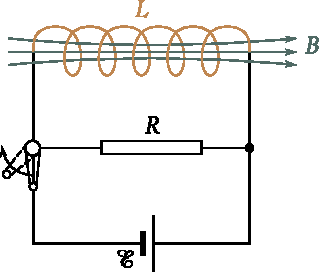
\includegraphics[scale=0.95]{figures/ch_08/fig_8_11.pdf}
		\caption[]{}
		\label{fig:8_11}
	\end{center}
	\vspace{-0.8cm}
\end{figure}

Nếu độ tự cảm của cuộn solenoid không phụ thuộc vào $I$ ($L=\text{constant}$), khi đó $\deriv{\Psi}=L\,\deriv{I}$, và \eqn{8_34} trở thành
\begin{equation}\label{eq:8_35}
	\deriv{A} = - LI\, \deriv{I}.
\end{equation}

\noindent
Tích phân biểu thức theo biến $I$ với cận từ $I$ đến không, ta thu được công mạch điện tác dụng để triệt tiêu hết từ trường là:
\begin{equation}\label{eq:8_36}
	A = - \int_I^0 LI\, \deriv{I} = \frac{LI^2}{2}.
\end{equation}

Công \eqref{eq:8_36} được truyền lại cho sự toả nhiệt của điện trở mạch, bao gồm $R$, cuộn solenoid, và dây nối.
Vì không có thay đổi nào khác xảy ra trong môi trường xung quanh mạch, chúng ta vẫn có thể kết luận rằng từ trường là thứ, và chính xác là công do\eqn{8_36} tạo ra.
Do đó, chúng ta kết luận rằng một vật dẫn có độ tự cảm $L$ có dòng điện $I$ chạy qua mang năng lượng
\begin{equation}\label{eq:8_37}
	W = \frac{LI^2}{2},
\end{equation}

\noindent
Năng lượng này có dạng biểu thức tương đối giống với năng lượng của một tụ điện lý tưởng tích điện $CU^2/2$; xem \eqn{4_5}].

Phương trình \eqref{eq:8_36} có thể được hiểu là công được thực hiện để chống lại suất điện động tự cảm. khi dòng điện tăng từ $0$ đến $I$, đồng nghĩa với việc thiết lập một từ trường có năng lượng cho bởi \eqn{8_37}.
Công chống lại suất điện động tự cảm là
\begin{equation*}
	A' = \int_0^I (-\ab{\mathcal{E}}{s}) I\, \deriv{t}.
\end{equation*}

\noindent
Biến đổi tương tự cũng đưa tua đến \eqn{8_35}, ta có
\begin{equation}\label{eq:8_38}
	A' = \int_0^I LI\, \deriv{I} = \frac{LI^2}{2}.
\end{equation}

\noindent
Dòng điện được sử dụng hoàn toàn để tạo ra một từ trường tạo ra bởi các vòng dây.
Phương trình \eqref{eq:8_38} không tính đến công sử dụng bởi nguồn điện để làm toả nhiệt các vật dẫn trong thời gian dòng điện đạt giá trị ổn định.

Ta hãy biểu diễn năng lượng từ trường được cho bởi \eqn{8_37} qua các đại lượng riêng của từ trường.
Đối với solenoid dài vô hạn
\begin{equation*}
	L = \mu_0\mu n^2V,\quad H=nI,\quad\text{or}\quad I=\frac{H}{n}
\end{equation*}

\noindent
[xem \eqn{7_29} và \eqn{8_14}].
Sử dụng các giá trị của $L$ và $I$ trong \eqn{8_37} và thực hiện các phép biến đổi liên quan, ta thu được
\begin{equation}\label{eq:8_39}
	W = \frac{\mu_0 \mu H^2}{2} V.
\end{equation}

Từ \sect{6_12} ta thấy rằng từ trường của một solenoid dài vô hạn là đồng nhất và chỉ khác 0 bên trong lòng ống solenoid.
Do đó, năng lượng cho bởi \eqn{8_39} phân bố chủ yếu bên trong lòng ống solenoid và có mật độ năng lượng $w$ được biểu diễn bằng việc chia $W$ cho $V$
\begin{equation}\label{eq:8_40}
	w = \frac{\mu_0 \mu H^2}{2}.
\end{equation}

\noindent
Sử dụng \eqn{7_17}, ta có thể viét ra mật độ năng lượng của từ trường trong lòng ống solenoid:
\begin{equation}\label{eq:8_41}
	w = \frac{\mu_0 \mu H^2}{2} = \frac{HB}{2} = \frac{B^2}{2 \mu_0 \mu}.
\end{equation}

Các biểu thức chúng ta thu được cho mật độ năng lượng của từ trường khác với Eqs. \eqref{eq:4_11} đối với mật độ năng lượng của điện trường chỉ khi các đại lượng tĩnh điện bên trong chúng đã được thay thế bằng các đại lượng từ trường liên quan.

Biết mật độ của năng lượng trường tại mọi điểm, chúng ta có thể tìm thấy năng lượng của từ trường bên trong một thể tích bất kỳ $V$.
Vì lý do này ta phải tính tích phân trên toàn không gian chứa từ trường
\begin{equation}\label{eq:8_42}
	W = \int_V w\, \deriv{V} = \int_V \frac{\mu_0 \mu H^2}{2}\, \deriv{V}.
\end{equation}

Đối với các vòng kết hợp (trong trường hợp không có sắt từ), năng lượng từ trường được xác định bởi phương trình
\begin{equation}\label{eq:8_43}
	W = \frac{L_1 I_1^2}{2} + \frac{L_2 I_2^2}{2} + \frac{L_{12} I_1 I_2}{2} + \frac{L_{21} I_2 I_1}{2}.
\end{equation}

\noindent
Một biểu thức tương tự thu được đối với năng lượng của các vòng $N$ được ghép nối tiếp với nhau:
\begin{equation}\label{eq:8_44}
	W = \frac{1}{2} \sum_{i,k=1}^N L_{i,k} I_i I_k,
\end{equation}

\noindent
với $L_{i,k}=L_{k,i}$ là độ hỗ cảm của vòng dây thứ $i$-th và $k$-th, và $L_{i,i}=L_i$ là độ tự cảm của vòng dây thứ $i$-th.

\section{Công nghịch từ của sắt từ}\label{sec:8_9}

Sự biến thiên của dòng điện trong mạch là kết quả của việc chống lại suất điện động tự cảm:
\begin{equation}\label{eq:8_45}
	\derivp{A} = (-\ab{\mathcal{E}}{s}) I\, \deriv{t} = \diff{\Psi}{t} I\, \deriv{t} = I\, \deriv{\Psi}.
\end{equation}

\noindent
Nếu độ tự cảm $L$ của mạch không đổi (chỉ khi không có sắt từ), công này chuyển hoá hoàn toàn thành năng lượng từ trường: $\derivp{A}=\deriv{W}$.
Bây giờ chúng ta sẽ nghiên cứu ảnh hưởng của chất sắt từ.

Đối với ống solenoid dài vô hạn, $H=nI$, $\Psi=nlBS$.
Khi đó,
\begin{equation*}
	I = \frac{H}{n},\quad \deriv{\Psi} = nlS\, \deriv{B}.
\end{equation*}

\noindent
Lắp vào \eqn{8_45}, ta thu được
\begin{equation}\label{eq:8_46}
	\derivp{A} = H\, \deriv{B} \times V,
\end{equation}

\noindent
với $V=lS$ là thể tích của solenoid, tức là, phần thể tích chứa từ trường mang năng lượng.

Ta sẽ xem \eqn{8_46} với sự tăng lên của năng lượng từ trường.
Tôi nhắc nhở người đọc rằng năng lượng là một hàm của trạng thái.
Do đó, tổng các gia số của nó cho một quá trình tuần hoàn bằng không:
\begin{equation*}
	\oint \deriv{W} = 0.
\end{equation*}

\noindent
Nếu lõi của solenoid được làm bằng sắt từ, thì mối liên hệ giữa $B$ và $H$ được mô tả bằng đường cong như \fig{8_12}.
Phần tử $H\,\deriv{B}$ là diện tích của phần được tô đậm trong hình.
Kết quả là, tích phân $\oint H\,\deriv{B}$ được tính dọc theo vòng từ trễ bằng diện tích $S_l$ được bao quanh bởi vòng dây.
Do đó, tích phân của biểu thức \eqref{eq:8_46}, tức là, $\oint\derivp{A}$, khác không.
Do đó nếu có mặt sắt từ, công do \eqn{8_46} đưa ra không bằng với độ tăng lên của năng lượng từ trường.
Sau khi hoàn thành chu kỳ đảo nghịch từ, $H$ và $B$ và, do đó, năng lượng từ trường sẽ quay về giá trị ban đầu.
Do đó, công $\oint\derivp{A}$ không chuyển hoá thành năng lượng từ trường.
Thực nghiệm cho thấy nó được dùng để tăng nội năng của chất sắt từ, tức là làm nóng nó lên

\begin{figure}[!h]
	\begin{center}
		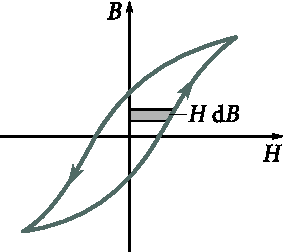
\includegraphics[scale=1]{figures/ch_08/fig_8_12.pdf}
		\caption[]{}
		\label{fig:8_12}
	\end{center}
	\vspace{-0.8cm}
\end{figure}

Do đó, việc hoàn thành một chu kỳ đảo chiều từ của một chất sắt từ được tham gia bởi công trên một đơn vị thể tích bằng với diện tích của vòng từ trễ:
\begin{equation}\label{eq:8_47}
	\ab{A}{u.vol} = \oint H\, \deriv{B} = S_l.
\end{equation}

\noindent
Công này làm nóng chất sắt từ

Nếu không có sự xuất hiện của sắt từ, $B$ là một hàm của $H$ ($B=\mu_0\mu H$, với $\mu=\text{constant}$).
Do đó, biểu thức $H\,\deriv{B}=\mu_0\mu H\, \deriv{H}$ là một vi phân
\begin{equation}\label{eq:8_48}
	\deriv{w} = H\,\deriv{B},
\end{equation}

\noindent
xác định sự tăng lên của năng lượng từ trường.
Tích phân của \eqn{8_48}với cận từ $0$ đến $H$ dẫn đến \eqn{8_40} cho mật độ của năng lượng từ trường (trước khi tích phân, $H\,\deriv{B}$ phải được biến đổi bằng cách thay $\mu_0\mu\,\deriv{H}$ với $\deriv{B}$).
